\documentclass[conference]{IEEEtran}
\usepackage{graphicx}

\begin{document}

% paper title
\title{Analysis of a Digital Non Linear System Implementation}


% author names and affiliations
% use a multiple column layout for up to three different
% affiliations
\author{\authorblockN{L. De Micco, M. Antonelli and H. A. Larrondo}
\authorblockA{Departamentos de F\'isica y de Ingenier\'ia Electr\'onica\\Facultad de Ingenier\'ia, Universidad
Nacional de Mar del Plata\\Juan B. Justo 4302, Mar del Plata,
Argentina and CONICET  Email: ldemicco@fi.mdp.edu.ar} }

 \maketitle



\begin{abstract}

This paper introduces an analysis of a fixed point implementation
of a multiatractor chaotic system. The aim of the analysis is to
find a threshold bus width where the system keep the desired
properties that the real one has. These properties depend on each
particular application, but here we determine a range of behavior.
The Shannon Entropy ($H$), applied to two different Probability
Density Functions (PDFs), and the Maximum Lyapunov Exponent
($MLE$) are the quantifiers employed here. These quantifiers
result to reflect the changes in period lengths of the system
output on a wide range of initial conditions (CIs).
%
%Beyond this threshold, the maximum Lyapunov exponent  is shown  to
%improve up to a peak value at 16-bits and subsequently decrease
%with increasing bus width. The MLE is also shown  to gradually
%increase  with number of introduced internal delay cycles until a
%peak value at 14 cycles, after  which the system loses chaotic
%properties. Introduced external  delay cycles are shown to rotate
%the attractors  in 3-D phase space. Bus width and delay elements
%can be independently modulated to optimize the system to suit
%specifications.




%In recent years chaotic systems became interesting because they
%may be used as controlled noise sources in many applications.  In
%digital implementations only pseudo chaotic systems are
%possible.
%It is not straightforward to design digital
%implementations preserving the pseudo chaotic nature, because of
%nonlinearity and extreme sensitivity to initial conditions.  Field
%Programmable Gate Arrays (FPGA) are the natural choice for digital
%implementations of a chaotic systems because they are
%reconfigurable allowing the design optimization and they can run
%faster than implementations in general purpose hardware.
%
%
%In a previous paper we analyzed the importance of the
%discretization of time and state variables, to increase the
%stochasticity of a chaotic system in order to use it as a pseudo
%stochastic source. Then we used the Euler algorithm for the FPGA
%implementations and considered:  (a) a fixed point architecture
%and (b) a floating-point single-precision IEEE $754$ standard
%architecture.
%
%
%The aim of this work is to
%
%A Lorenz chaotic system is used to exemplify the procedure and it
%fits onto an Altera EP3C120F7 FPGA board, using only $12$ \% of
%its logic elements and $34$ \%  of its memory bits. The provided
%design methodology can be applied to any continuous chaotic
%systems with minimal changes.

\end{abstract}

\IEEEpeerreviewmaketitle



%In the last thirty years chaotic systems have yielded a revolution
%in our vision about nature as they have two contrasting features: on the one hand, they have a mathematical model and then they are included in the \textsl{deterministic system} class; on the other hand because of the initial conditions sensitivity, the long time predictivity is lost and then they may also be included in the class of
%\textsl{stochastic systems} for which the analysis is performed by
%statistical means \cite{Beck1997, Lasota1994, Rosso2007A}. Actually, if chaotic systems could be
%implemented with infinite precision, they would be deterministic
%in the strict sense.
%
%%\smallskip
%Chaotic systems deterministic-stochastic duality make them
%specially interesting for engineering in a wide range of
%applications \cite{Fernandez2003, Stojanovski2001, Stojanovski2001b, Kocarev2003, Larrondo2005, DeMicco2007B, DeMicco2008} .
%
%One interesting application is the use of analogue chaotic generators in
%communication systems \cite{Kocarev2003, Fernandez2003}. Recovery of the information signal depends
%on the exact synchronization between the  receiver and the transmitter. It
%requires the parameters of both -receiver and transmitter- to be
%matched to a high degree of accuracy. This requirement is
%difficult to achieve in analogue systems because the values of
%analogue circuit component are functions of age and environmental conditions. A solution is to implement the chaotic generators using digital hardware.
%
%But in a digital application both time and value of signals
%are discrete. Time discretization forces the use of algorithms to
%replace the differential equations that model the system. Among
%the usual algorithms the simplest is first order Euler's method in
%which differentials are directly replaced by finite increments but more elaborated algorithms must be used if a better approach is required \cite{Press1995}. Discretization of signals is equivalent to define a finite
%alphabet and to convert the original series to a symbolic series
%(that in our case is also a numerical series). Thus, for example
%the $n$ bits integer arithmetic representation has a $2^n$ symbols
%alphabet and a floating point representation that depends on the
%standard adopted \cite{Gonzalez2005, DeMicco2010}.
%
%

%
%In a previous paper \cite{DeMicco2010,Gonzalez2003} the
%Lorenz oscillator was implemented with the Euler's algorithm
%(discretization of time) and in two different numerical
%representation (discretization of signals):  fixed point
%arithmetics and floating- point single-precision IEEE $754$
%standard. Those representations are convenient when the chaotic
%system is used as a controlled noise source. We present here results for the same dynamical system but with a higher precision, using the fourth order Runge$-$Kutta algorithm with floating-point single-precision IEEE $754$ standard architecture to discretize the state variables.
%
%A Lorenz chaotic system is used to exemplify the procedure and it fits onto an Altera EP3C120F7 FPGA board, using  only $12$ \% of its logic elements and $34$ \%  of its memory bits.
%The provided design methodology can be applied to any continuous chaotic systems with minimal changes.
%The implementation was fully done with $Quartus$ II
%$7.2^\copyright$ development software. The simulation and physical
%implementation on an $Altera^\copyright$ Cyclone III $EP3C120$
%development kit. Results are compared with those obtained
%previously with Euler's method in: (a) $16$ bits integer
%arithmetic \cite{Gonzalez2003} and, (b) floating point single
%precision \cite{DeMicco2010}.
%

\section{Introduction} \label{sec:intro}

Digital implementation in hardware of systems forces the usage of
 finite number of bits to represent the state variables' values.

Floating point architecture allows to recreate the system's
trajectories close to the real (ideal) ones.

However, from the engineering point of view the usage of floating
point arithmetic is not efficient when compared to fixed point
operations because the first ones consume lot of system
resources and require several clock cycles.

If the system to be implemented is known, i.e. the maximal values
of its variables and the precision required are pre-established,
fixed point arithmetic would allow to get better results in terms
of velocity, usage resources and power consumption.

In general, for linear systems the digitalization process is not a
defining issue since, roughly, linear systems remain almost their
 behavior. Therefore, discretized values can be modelled with a small noise called \textit{quantization noise}.

In nonlinear systems the necessary amount of bits for representing
the integer and fractional part of each value is critical. This is
because of the high sensitivity of the systems that provokes to
totally change their dynamics. The integer part is easily
determined by the maximum value that the system could reach, and
its optimum value can be rapidly found by a fast analysis. On the
other hand, the number of bits needed for representing the
fractional part is determined by the required accuracy.

In this systems by varying the precision used, completely
different behaviors are obtained, from unstable systems to
converging to fixed points, and within a range, a good
approximation to the real system.

Several strategies can be used for selecting the optimal amount of
bits for hardware implementations. However, the methods proposed
in the literature are limited to linear systems
\cite{Constantinides2002,Constantinides2003}.

Recently, hardware implementation of chaotic oscillators has
gained interest and several new schemes have been proposed
\cite{Qun2007,Aseeri2002,Azzaz2009}.

In the literature, there does not seem to be much work on
quantitative analysis of the degradation due to digitalization of chaos and
how to reduce its negative influence on chaos-based digital
systems. Grebogi's work \cite{Grebogi1988} showed that the average
length of periodic orbits (T) of a dynamical system scales as a
function of computer precision (e) and the correlation dimension
(d) of the chaotic attractor: $T \sim  e^{-d/2}$. In
\cite{SHUJUN2005} some findings on a new series of dynamical
indicators, which can quantitatively reflect the degradation
effects on a digital chaotic map realized with a fixed-point
finite precision have been reported. They are restricted to $1D$
piecewise linear chaotic maps (PWLCM).

In this work we developed a detailed analysis of a fixed point implementation
of a multiatractor chaotic system. The aim of the analysis is to find a threshold
bus width where the system keep the desired properties that the real one has.

Of course these properties depend on each particular application,
but here we determine a range of behaviour. The Maximum Lyapunov
Exponent and the Normalized Shannon Entropy are the quantifiers
employed here, they are applied to two different PDFs. This
quantifiers result to reflect the changes in period lengths of the
system output on a wide range of initial conditions.


The work is organized as follows: in section \ref{sec:estudio} an
analysis of the allowed initial conditions of the system is
performed. Section \ref{sec:caos} gives a brief description of the
chaotic system analyzed, and a detailed explanation of how the
digitalization is performed.

Section \ref{sec:Quantifiers} theoretical background of the quantifiers employed here.

Section \ref{sec:repre} describes our proposed method in detail.
We give experimental result in Section \ref{sec:resultads}.

Finally, the conclusions and future work are given in section
\ref{sec:conclusiones}.


\section{Attraction domain analysis} \label{sec:estudio}

Generally, the usefulness of the nonlinear systems implementations
are the ``random" generated sequences to be employed as controlled
noises generators (PRNGs), encryption sequences for privacy,
multiplexing techniques, and so on. For this reason, unpredictable
long periods are desired.

In this way, it is necessary to know the seeds, i. e. initial
conditions, that generate random-like outputs of the system and
also the degree of ``randomness".

In the universe of all the possible initial conditions, some
converge to attractors (this group is called the attractor domain)
and the remaining points diverge, go to infinity.

An attractor is a point or a collection of points on which the
system limits. When using finite precision these take the form of
fixed points and periodic orbits.

If the precision employed is adequate, attractors of really long
periods can be reached. Moreover the ``randomness" degree of the
sequences must be taken into account, to this aim we have employed
some quantifiers (section \ref{sec:Quantifiers}).

\subsection{Chaotic System analyzed}\label{sec:caos}

With the purpose of showing the method of analysis it has been chosen a family of bi-dimensional quadratic maps which
structure consists of a pair of coupled quadratic difference
equations (eq. \ref{eq:Quad-map}) to be analyzed. Its $12$
coefficients correspond to the parameters of the chaotic system.
The main characteristic of this system is that each set of
parameters $a_n$, produces a different evolution of it. This is
called \textit{multiattractor}, and means that the chaotic
behavior of the system changes with the parameters values. Fig.
\ref{fig:atractores} shows three different attractors that
correspond to three different sets of parameters.
%%%%%%%%%%%%%%%%%%%%%%%%%%%%%%%%%%\cite{Antonelli uEA2012}.(Maxi)

{ \small
\begin{eqnarray}\label{eq:Quad-map}
    x_{(i+1)}&=& a_0 + a_1 x_{(i)} + a_2 x_{(i)}^2 + a_3 x_{(i)} y_{(i)} + a_4 y_{(i)}^2 + a_5 y_{(i)} \nonumber\\
    y_{(i+1)}&=& a_6 + a_7 x_{(i)} + a_8 x_{(i)}^2 + a_9 x_{(i)} y_{(i)} + a_{10} y_{(i)}^2 + a_{11} y_{(i)}\nonumber\\
\\
\nonumber \end{eqnarray}

}
%%%%%%%%%%%%%%%%%%%%%%%%%%Ver por que queda mal centrado el n�mero(Maxi)

\begin{figure}
    \centering
    \includegraphics[width=1\columnwidth]{atractoreslindos.jpg}\\
    \caption{Three attractors for three different values of the coefficients {$a_n$}.}\label{fig:atractores}
\end{figure}


The system behavior in real arithmetic has been widely studied, however
real variables are not possible to implement in hardware, so
finite precision operations should be employed.

The utilization of finite number of bits limits the quantity of
available symbols used to represent the state variables.
Therefore, finite arithmetic implies that the implemented system
will always have a finite repetition period, and it will be
determined when all the state variables, in this case $x$ and $y$,
repeat their values. Accordingly, the maximum theoretical period
that can be reached is determined by the quantity of bits of all
the state variables, and is: $2^{(\sharp
{state\_variables*n_{bits})}}$ , where $n_{bits}$ is the bus width
and $\sharp state\_variables$ is the quantity of states variables
of the system.

For example if we use $10$ bits for the numeric representation
($n_{bits} =10$), the maximum theoretical period would be
$2^{(2*10)} = 1048576$. Actually, the periods obtained are in
general lower than the theoretical one and they depend on the
initial condition of the sequence.

In Fig. \ref{atrac} the attraction domain scheme of the system for
parameters:
\small{$a_n={-1,0.9,0.4,-0.2,-0.6,-0.5,0.4,0.7,0.3,-0.5,0.7,-0.8}$}
can be seen. Axes $x$ and $y$ are the values of the initial
conditions. In chaotic systems all initial conditions within the
basin of attraction look the same after many iterations. The grey
colored area are the points of all the initial conditions that,
after a transient, converge to the attractor, which has been
highlighted in black color.

\begin{figure}
    \centering
    \includegraphics[width=1.1\columnwidth]{atractorcondimension1.jpg}\\
    \caption{Atraction Domain and attractor of the system analyzed.}\label{atrac}
\end{figure}

\subsection{Analysis of sequences' periods}

As mentioned above, digitalization changes the statistical
properties of the implemented systems. Because of this fact, it is
necessary to check that the system still satisfies the
application's requirements.

We have systematically studied the behavior of the system's output
using different precisions in a fixed point architecture,
emulating a FPGA implementation. This was done for various initial
conditions in order to obtain the attraction domain scheme of the
system. Our interest is to understand how the attraction domain
evolves with the variation of the bits employed in the precision,
and also to find a threshold value above which the chaotic
behavior of the system appears.

To this aim we have employed different quantifiers, the Normalized
Shannon Entropy applied to two different probability density
functions, and the Maximum Lyapunov Exponent that determines the
presence of chaos.

%If you choose initial values of X and Y somewhere near the
%attractor, within its basin of attraction, and substitute these
%values into the equations that describe the attractor, the new
%values of X and Y represent a point in the plane that is closer to
%the attractor. After a number of iterations, the point works its
%way to the attractor, and thereafter it moves around on the
%attractor in some complicated manner, eventually visiting every
%part of the attractor. The next position can always be simply and
%accurately predicted from the current position, but the small,
%inevitable uncertainty in position continually increases so that a
%long term prediction is impossible, except to say that the point
%is somewhere on the attractor. You can think of the attractor as
%the set of all possible long-term solutions of the equations that
%produced it.
%
%Besides the error in knowing perfectly the initial conditions,
%there are also computer round-off errors at each iteration. Given
%the extreme sensitivity to small errors, you may wonder whether
%any computer is capable of calculating correctly such a chaotic
%process. It is true that if the same chaotic equations are
%iterated on two computers using different precision or round-off
%methods, the sequence of iterates is almost certainly completely
%different after a few dozen iterations. However, the appearance of
%the attractor is probably the same. In such a case, we say that
%the solution is structurally stable or robust. Furthermore,
%according to the shadowing lemma, an appropriate small change in
%initial conditions produces a chaotic sequence that follows
%arbitrarily close to the computed one.
%
%Since computers always round the results of calculations to a
%finite number of digits (or more precisely, bits), a limited
%number of values is allowed. Thus successive iteration of a map
%always eventually repeats a previously obtained value, whereupon
%the solution reproduces exactly the same sequence of states as it
%did before. Strictly speaking, every such solution is periodic,
%and true chaos cannot be observed with a computer. However, with
%double-precision floating point variables, which are normally 64
%bits, there are 264 or about 1019 possible values. It can be shown
%that an average periodicity occurs after about the square root of
%this number of iterations, which is about 3 x 109. Until the
%number of iterations approaches this value, there is little cause
%to worry. For maps higher than one dimension, this problem is even
%less serious because all the variables have to reach a previously
%existing state at the same time.

\section{Quantifiers}
\label{sec:Quantifiers}

In the present work we compare the results of employing various
precision using two type of quantifier that have demonstrated to
accurately differentiate between various systems. One comes from
the Information Theory, the Shannon Entropy, that after a proper
evaluation of PDF is made by recourse to one of the two distinct
approaches in coordinate space, namely, {\it (i)  \/} the
Bandt-Pompe technique, and {\it (iii)\/} PDF based on histograms;
The Maximum Lyapunov Exponent characterizes how fast two
trajectories drift apart, if this rate is exponential the system
is said to be chaotic, because of this it is known as a detector
of ``chaoticity", \cite{strotgartz1994,Kantz1994,Sprott2003}.

\subsection{Shannon Entropy}
%
% agregado en borrador de hilda
Any discrete alphabet time series has two important properties:
(1) the list of elements of the alphabet and the probability of
each element, and (2) the order of the elements inside the time
series (mixing). Each property my be characterized by means of
probability distribution functions  $P = \{ p_j, j=1, \cdots, N
\}$ and their corresponding entropies. To evaluate (1) it is
possible to use the normalized histogram of the time series as a
PDF. Once the PDF is known the entropy is defined by the very well
known Shannon expression:

\begin{eqnarray}
S[P]~=~-\sum _{j=1}^{N}~p_j~\ln( p_j ), \nonumber\\
H[P] = {\rm S}[P]~/~{\rm S}[P_e]. \label{eq:shannon}
\end{eqnarray}

With $P_e $ being the uniform  distribution and $N$  the number of
possible states of the system under study.




% falta que termine este pedazo

\subsubsection{PDF based on Band and Pompe methodology}

To use the Bandt and Pompe \cite{Pompe} methodology for evaluating
of probability distribution $P$ associated to the time series
(dynamical system) under study one starts by  considering
partitions of the pertinent $D$-dimensional space that will
hopefully ``reveal" relevant details of the ordinal-structure of a
given one-dimensional time series $ \{x_t : t=1, \cdots,M \}$ with
 embedding dimension $D > 1$. We are interested in ``ordinal
patterns" of order $D$ \cite{Pompe,Keller} generated by
\begin{equation}
(s)~\mapsto~
\left(~x_{s-(D-1)},~x_{s-(D-2)},~\cdots,~x_{s-1},~x_{s}~\right) \
, \label{vectores}
\end{equation}
which assign to each time $s$ the $D$-dimensional vector of values
at times $s, s-1,\cdots,s-(D-1)$. Clearly, the greater the
$D-$value, the more information on the past  is incorporated into
our vectors. By the ``ordinal pattern" related to the time $(s)$
we mean the permutation $\pi=(r_0,r_1, \cdots,r_{D-1})$ of
$(0,1,\cdots,D-1)$ defined by
\begin{equation}
x_{s-r_{D-1}}~\le~x_{s-r_{D-2}}~\le~\cdots~\le~x_{s-r_{1}}~\le~x_{s-r_0}
\ . \label{permuta}
\end{equation}
In order to get a unique result we set $r_i <r_{i-1}$ if
$x_{s-r_{i}}=x_{s-r_{i-1}}$. Thus, for all the $D!$ possible
permutations $\pi$ of order $D$, the probability distribution
$P=\{p(\pi)\}$ is defined by
\begin{equation}
p(\pi)~=~\frac{\sharp \{s|s\leq M-D+1;~ (s) \texttt{, has type
}\pi\}}{M-D+1} \ . \label{frequ}
\end{equation}
In this expression, the symbol $\sharp$ stands for ``number".


The Bandt-Pompe's methodology is not restricted to time series
representative of low dimensional dynamical systems but can be
applied to any type of time series (regular, chaotic, noisy, or
reality based), with a very weak stationary assumption (for $k =
D$, the probability for $x_t < x_{t+k}$ should not depend on $t$
\cite{Pompe}). One also assumes that enough data are available for
a correct attractor-reconstruction. Of course, the embedding
dimension $D$ plays an important role in the evaluation of the
appropriate probability distribution because $D$ determines the
number of accessible states $D!$. Also, it conditions the minimum
acceptable length $M \gg D!$ of the time series that one needs in
order to work with a reliable statistics.

\subsubsection{PDF based on histograms}

In order to  extract a PDF via amplitude-statistics, divide first
the interval $[0,1]$ into a finite number $nbin$ of non
overlapping subintervals $A_i$: $[0,1]=\bigcup_{i=1}^{nbin} A_i$
and $A_i\bigcap A_j=\emptyset~\forall i\neq j$. One then employs
the usual histogram-method, based on counting the relative
frequencies of the time series values within each subinterval. It
should be clear that the resulting  PDF lacks any information
regarding temporal evolution. The only pieces of information we
have here are the $x_i-$values that allow one to assign inclusion
within a given bin, ignoring just where they are located (this is,
the subindex $i$.)

\subsection{Maximum Lyapunov Exponent}

The Lyapunov exponents are quantifiers that characterize how the
separation between two trajectories evolves, \cite{Sprott2003}. It
is generally well known that chaotic behaviors are characterized
mainly by Lyapunov numbers of the dynamic systems. If one or more
Lyapunov numbers are greater than zero, then the system behaves
chaotically, otherwise, the system is stable. In this paper, we
employ the maximum Lyapunov number as it is one of the most useful
indicators of chaos.

The distance between trajectories changes in $2^{MLE}$ for each
iteration, on average. If $MLE<0$ the trajectories approaches,
this may be due to a fixed point, if $MLE=0$ the trajectories keep
their distance, this may be due to a limit cycle, if $MLE>0$, the
distance between trajectories is growing, and is an indicator of
chaos. \cite{Sprott2003}

There is a non-analytical way to measure it if only the inputs and
outputs of the system are accessible. The procedure is the
following: The system must be started from two neighbor points in
the phase plane, lets call them $(x_a,y_a)$ and $(x_b,y_b)$, as
the system is iterated the Euclidean distance between the two
trajectories is measured ($d_n$ in the $n_{th}$ sample) (eq.
\ref{eq:D0D1}), and the b trajectory is relocalized on each
iteration  (eq. \ref{eq:reubicacion}), obtaining the points
$(x_{br},y_{br})$ to feed the system. Then the Lyapunov exponent
can be calculated as shown in eq. (\ref{eq:Lyapunov}). The process
can be seen in Fig. \ref{fig:relocalizacion}.


\begin{eqnarray}\label{eq:D0D1}
    d_{0(i-1)}&=& \sqrt{(x_{a(i-1)}-x_{br(i-1)})^2+(y_{a(i-1)}-y_{br(i-1)})^2}\nonumber\\
    d_{1(i)}&=& \sqrt{(x_{a(i)}-x_{b(i)})^2+(y_{a(i)}-y_{b(i)})^2}\\
\nonumber
\end{eqnarray}

\begin{eqnarray}\label{eq:Lyapunov}
    MLE &=& \frac{1}{M} \sum_{i=2}^{M} \log_2{\frac{d_{1(i)}}{d_{0(i-1)}}}
\end{eqnarray}


\begin{eqnarray}\label{eq:reubicacion}
    x_{br(i)}&=& x_{a(i)}+(x_{b(i)}-x_{a(i)})d_{o(i-1)}/d_{1(i)} \nonumber\\
    y_{br(i)}&=& y_{a(i)}+(y_{b(i)}-y_{a(i)})d_{o(i-1)}/d_{1(i)}
\end{eqnarray}


\section{Hardware Digital simulation.} \label{sec:repre}

A \textit{C} code that simulates a nonlinear system was developed.
In this case the quadratic map was reproduced as it would be
implemented in a digital hardware dispositive, for example a FPGA
implementation. The Code employs signed integer arithmetic and it
is equivalent to employ fixed point precision.


The system is intended to be working in decimal fixed point
architecture. It employs $4$ bits for representing the integer
part in $Ca_2$ convention ($m=4$) and it automatically scans the
number of bits to represent the fractional part of the number (n),
in order to analyze how the system reacts when the precision
changes.


For example in Table \ref{tab:tabla} there is the equivalence when
using $n_{bits} =6$, $4$ bits for the integer part and $2$ bits
for the decimal part in $Ca_2$ convention ($m=4$ and  $n=2$).

\begin{table}[h]
  \caption{Table of equivalences.}\label{tab:tabla}
  \vspace{2mm}
  \centering
  \begin{tabular}{ c c c }
  Binary  & Decimal Fixed point & Signed Integer  \\
   \hline
  $0111,11$ & $7,75$ & $31$ \\
  $0111,10$ & $7,5$ & $30$ \\
  $0111,01$ & $7,25$ & $29$ \\
   ... & ... &  ...\\
  $0000,00$ & $0$ & $0$  \\
  $1111,11$ & $-0,25$ & $-1$ \\
  $1111,10$ & $-0,5$ & $-2$  \\
   ... & ... & ... \\
    $1000,00$ &  $-8$ & $-32$  \\
  %  \hline
    \end{tabular}
\end{table}



Internally the FPGA works with binary numbers, designers must
interpret the bits based on the desired architecture. In order to
use the parameterizable operations provided by the FPGA's
libraries, that work with Signed Integer variables, an equivalence
between Decimal fixed point numbers and Signed Integers can be
done as shown in Table \ref{tab:tabla}.

The same binary number can be interpreted as an integer number or,
as in this case, if one wish to employ decimal numbers, interpret
a decimal point located at a desired position. This means:

\begin{equation}\label{eqdecimal}
number=-2^{(m-1)} ... 2^0,2^{-1}�2^{-n}
\end{equation}

where $n\_bits=m+n$.

In order to make this conversion, each decimal number must be
multiplied by $2^n$ to obtain the equivalent Signed Integer
number. Where $n$ is the quantity of bits used to represent the
decimal part of the number. This is equivalent to right-shift $n$
positions the decimal point.

\begin{equation}\label{eqentero}
 number= -2^{(m-1+n)} ... 2^0
\end{equation}

where $n\_{bits}=m+n$.

The following considerations must be taken into account when operating with this equivalence:

\begin{itemize}
    \item Addition, this operation does not need any consideration just to make sure not to exceed the limits of the arithmetic used.
    \item Multiplication, the result of this operation must be divided by $2^n$ to adjust the result to the correct range.
    \item Division, the result must be always rounded towards minus infinity: $7.28$ to $7$ , $-14.9$ to $-15$.
\end{itemize}


The developed code iterates the Quadratic map (eq.
\ref{eq:Quad-map}) with the following coefficients: \small{
$a_0=-1.0$, $a_1= 0.9$, $a_2= 0.4$, $a_3= -0.2$, $a_4= -0.6$,
$a_5= -0.5$, $a_6= 0.4$, $a_7= 0.7$, $a_8= 0.3$, $a_9=-0.5$,
$a_{10}= 0.7$ and $a_{11}= -0.8$}.


Hence, the operations are done using signed integer variables that
are equivalent to decimal fixed point numbers, as it has been
explained in the previous section.

After each operation the corresponding adjustment is performed to work exactly as the FPGA does.


The map has been iterated with initial conditions $x_0$ and $y_0$
from  $-2$ to $2$ in steps of $0.001$, that means $16008001$
different points. On each case it was determined whether the
systems evolves to a fixed point, diverges or goes towards a
periodic cycle. It was also reported the repetition period of
these cycles.


For every value of precision $n$ we obtained a $4001$x$4001$ matrix whose elements correspond to each
initial condition. This means, the program outputs on each
position the final state of the system for that initial condition.

There are some desirable properties that constitutes a ``good"
PRNG, some of the most important ones are large period, few fixed
points and, of course, that do not diverge.

\section{Results} \label{sec:resultads}

Figures \ref{m5otro} to \ref{m16otro} display some of the results
(i.e. for some values of $n$) obtained, these are the set of final
states for each initial condition. With final state we mean: fixed
point, divergent point or the value of the period when the CI
converges to a cycle.

The abscissa and ordinate axis correspond to initial values of $x$
and $y$ respectively. They have been swept from $-2$ to $2$ in
steps of $0.001$.

It can be seen that for small values of $n$ the zone presents
bigger areas of divergent and fixed points. As the value of $n$
increases, it can be seen that the area of divergent points tends
to the one of the floating point (Fig. \ref{atrac}).

Lower values of $n$ present rough surfaces, with predominant dark
colors indicating that there is a prevalence of
 short periods cycles. As the value of $n$ increases the area smoothes and the
color tends to be lighter, indicating that the CIs converge to
higher periods cycles. This means that the range of initial values
that generate useful sequences increases for higher values of $n$.

Also, it is interesting to note that the edges of the attraction
domain is irregular for small values of $n$, and it defines as $n$
increases.

\begin{figure}
    \centering
    \includegraphics[width=0.8\columnwidth]{Mapa2_m5.jpg}\\
    \caption{Domains of attraction $n=5$}\label{m5otro}
\end{figure}

\begin{figure}
    \centering
    \includegraphics[width=0.8\columnwidth]{Mapa2_m6.jpg}\\
    \caption{Domains of attraction $n=6$}\label{m6otro}
\end{figure}

\begin{figure}
    \centering
    \includegraphics[width=0.8\columnwidth]{Mapa2_m7.jpg}\\
    \caption{Domains of attraction $n=7$}\label{m7otro}
\end{figure}

\begin{figure}
    \centering
    \includegraphics[width=0.8\columnwidth]{Mapa2_m10.jpg}\\
    \caption{Domains of attraction $n=10$}\label{m10otro}
\end{figure}

\begin{figure}
    \centering
    \includegraphics[width=0.8\columnwidth]{Mapa2_m11.jpg}\\
    \caption{Domains of attraction $n=11$}\label{m11otro}
\end{figure}



\begin{figure}
    \centering
    \includegraphics[width=0.8\columnwidth]{Mapa2_m14.jpg}\\
    \caption{Domains of attraction $n=14$}\label{m14otro}
\end{figure}

\begin{figure}
    \centering
    \includegraphics[width=0.8\columnwidth]{Mapa2_m16.jpg}\\
    \caption{Domains of attraction $n=16$}\label{m16otro}
\end{figure}

An analysis of these outputs can be seen in Figures
\ref{puntosfijos} to \ref{periodosmaximos}.

Fig. \ref{puntosdivergentes} and  \ref{puntosfijos} show the
quantity of points that diverge and converge to fixed points
respectively as the value of $n$ increases, in both cases the
final value tends to the floating point case. It is clear from
these figures that for $n \sim 12$ the system seems to behave
sufficiently accurate to the real one. However Figure
\ref{periodosmaximos} shows that a value of $12$ for $n$ the
system still have a quite short maximum period.

\begin{figure}
    \centering
    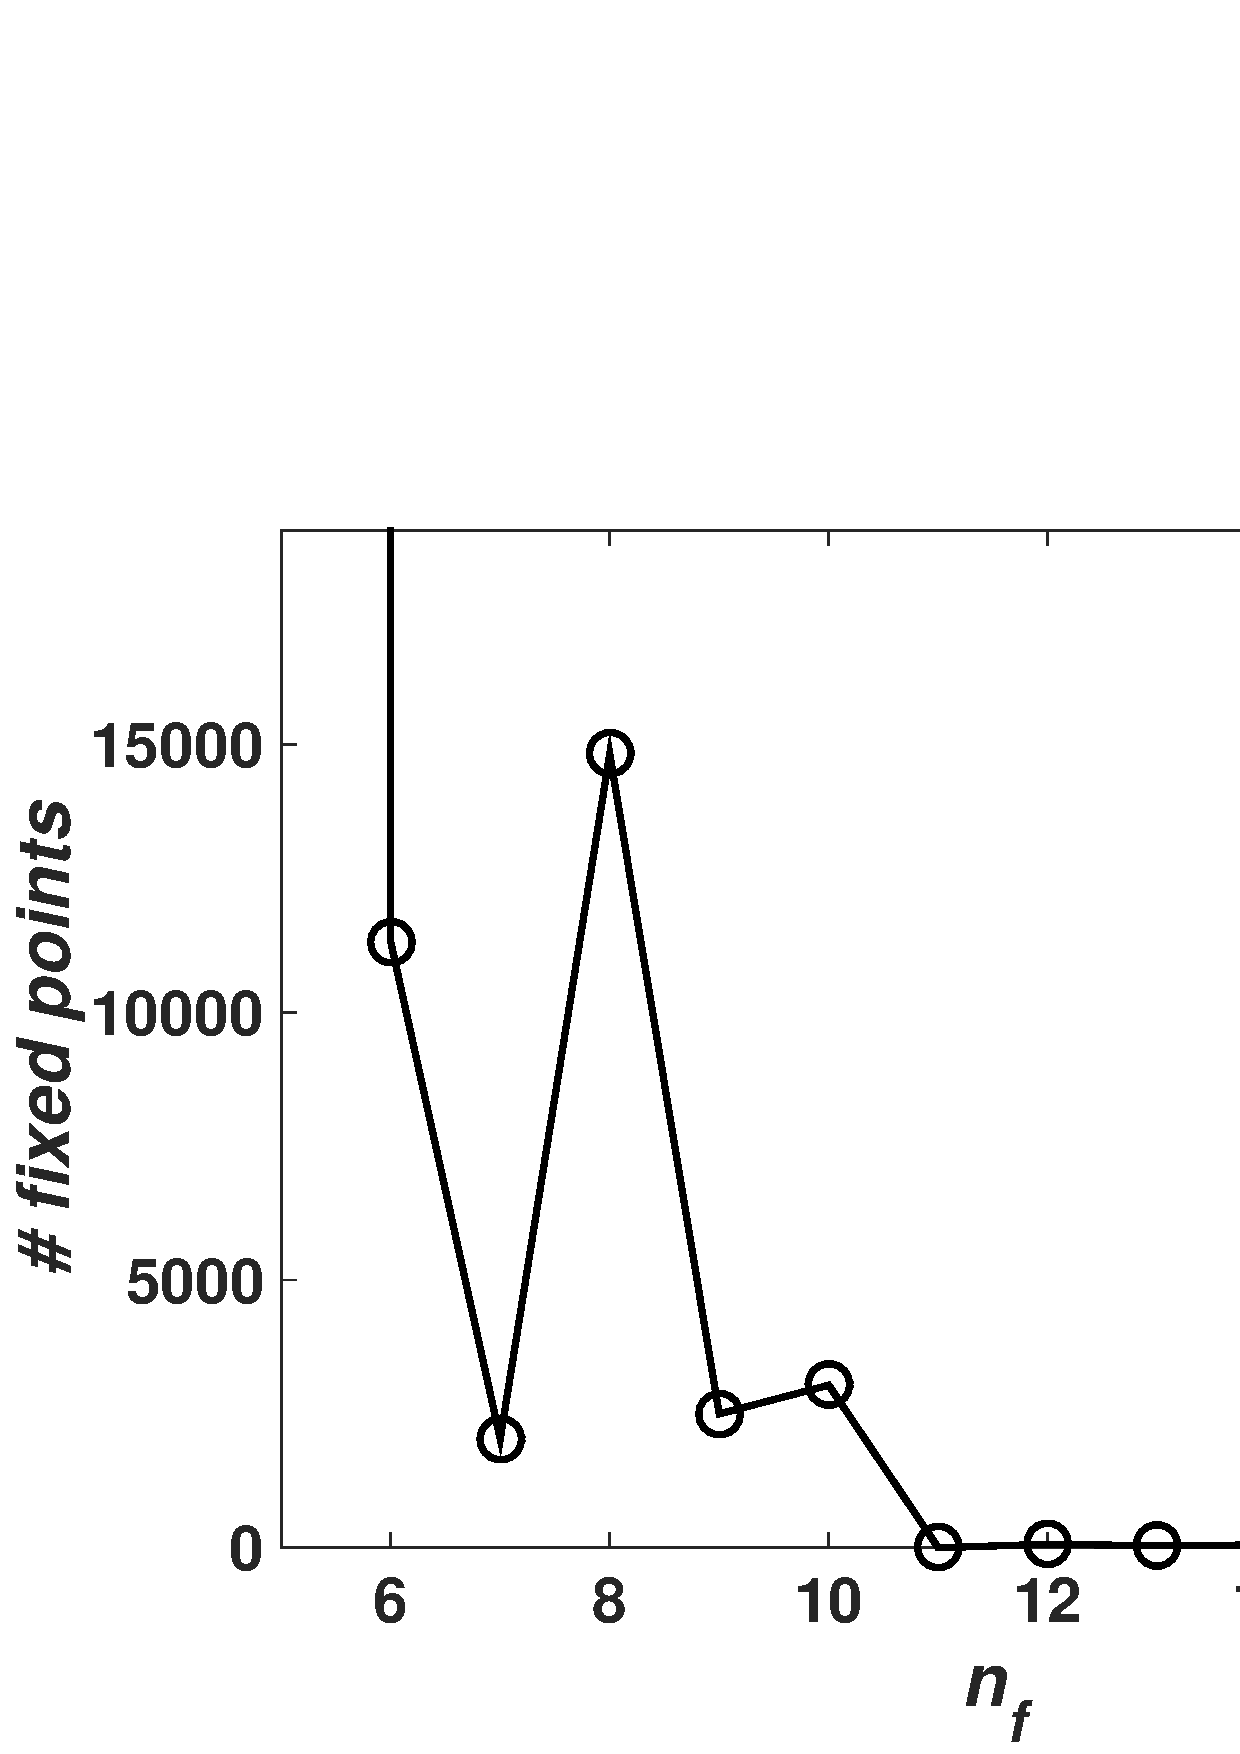
\includegraphics[width=0.7\columnwidth]{ptosfijos.jpg}\\
    \caption{Quantity of fixed points.}
    \label{puntosfijos}

\end{figure}

\begin{figure}
    \centering
    \includegraphics[width=0.7\columnwidth]{divergen.jpg}\\
    \caption{Quantity of divergent points.}\label{puntosdivergentes}

\end{figure}

\begin{figure}
    \centering
        \includegraphics[width=0.7\columnwidth]{periodosmaximos.jpg}\\
    \caption{Maximum periods reached.}\label{periodosmaximos}

\end{figure}




\begin{figure}
    \centering
        \includegraphics[width=0.9\columnwidth]{Puntos.jpg}\\
    \caption{Quantity of initial conditions with period ($T$) higher and lower than $1000$.}\label{puntos}

\end{figure}



\begin{figure}
    \centering
        \includegraphics[width=0.9\columnwidth]{HBP_Hhist.jpg}\\
    \caption{Quantifiers $H_{BP}$  and $H_{hist}$.}\label{HBPHhist}

\end{figure}


Figure \ref{puntos} shows the quantity of initial conditions that
presents periods $T$ higher and lower than $1000$. Again, a value
of $12$ for $n$ seems to be the limit to obtain a good
approximation of system.

%
% this is
%interesting because in many applications these maps are intended
%to be used as controlled noise generators. So, to ensure long
%periods is required.
We realized that the analysis performed up to this point was not
enough to determine a conclusion, so we decided to further
analysis the data obtained by employing some statistical
quantifiers the Entropy applied to the $hist$ and $Band and Pompe$
distributions. Figure \ref{HBPHhist} shows the values of the
quantifier normalized Shannon entropy applied over two PDFs, the
histogram ($H_{hist}$) and Bandt-Pompe distribution ($H_{BP}$). In
the figure it can be seen that the two quantifiers tend to the
value calculated using floating-point arithmetic. While $H_{BP}$
is concordant with the previous analysis and shows that it
stabilizes for $n \sim 12$, $H_{hist}$ reaches the theoretical
value for $n \sim 19$, showing that there are properties of the
output sequences that only this quantifier can detect.

In Table \ref{MLE} the value of $MLE$ for some values of $n$. The
cases for $n=11, 12, 13$ and $25$ are showed. Also, the
theoretical value calculated with Matlab using floating point
arithmetic. It can be seen that as the value of $m$ increases the
$MLE$ tends to the theoretical value. Figure \ref{MLE} displays
 $MLE$ vs. $n$, there again the quantifier reaches the theoretical value at $n \sim 13$.

\centering

\begin{tabular}{|c|c|}

  \hline\label{MLE}

  n & MLE \\
  \hline
  $11$ & $0.049214459144086$ \\
  $12$ & $0.107498218078192$ \\
  $13$ & $0.139472468153184$ \\
  $14$ & $ 0.135756935006498$ \\
  $15$ & $0.144155039896011$ \\
  $16$ & $0.137514471652835$ \\
  $25$ & $0.142134613438658$ \\
  $27$ & $0.141180317168284$ \\
  float & $0.142275657734227$ \\
   \hline

\end{tabular}

\begin{figure}
    \centering
        \includegraphics[width=0.9\columnwidth]{Lyapunov.jpg}\\
    \caption{$MLE$ for different quantity of decimal bits $n$.}\label{MLE}

\end{figure}

\section{Conclusion} \label{sec:conclusiones}
The results show that, compared to floating-point, fixed-point
arithmetic executed on an integer datapath has a limited impact on
the accuracy.
%A new method to design chaotic generator models in real time is
%introduced which is capable of implementing the chaotic systems
%that are given by state equations in real time using FPGA system.
%The method is implemented by Quartus II software.
%
%In future implementations we may use more complex methods of
%integration in order to assess the accuracy of numerical
%integration so as to improve the accuracy obtained. We will employ
%variable step Runge$-$Kutta, Adaptive Stepsize Control and Verlet
%integration.

\section*{Acknowledgment}
% optional entry into table of contents (if used)
%\addcontentsline{toc}{section}{Acknowledgment}

This work was partially financed by CONICET (PIP2008),  and UNMDP.

\bibliographystyle{unsrt}
\bibliography{xbibWEBjun2012_ingles}
%\bibliographystyle{unsrt}
%\bibliography{xbibWEBjmayo2013_ingles.bib}


% that's all folks
\end{document}
